% =============================================================================
% Section 1 — Reading a Proof About a Cell
% =============================================================================
\section{Reading a Proof About a Cell}\label{sec:proof-and-cell}

\begin{objectives}
\begin{itemize}[leftmargin=*,itemsep=1pt,topsep=1pt]
  \item State precisely what a machine-checked proof establishes about a biological claim, and what it leaves untouched.
  \item Separate the three independent things that can go wrong in a quantitative claim: the arithmetic, the model, and the measurement.
  \item Read and write an \emph{epistemic ledger}, the device used at the end of every section of this book.
  \item Explain why a theorem can be perfectly true and the biology it describes still false.
\end{itemize}
\end{objectives}

\subsection{Three ways to be convinced, and why you need all of them}

Suppose someone tells you that a particular mutation in a DNA polymerase raises a
tumour's mutation count by a factor of seven thousand. Before believing it, ask
which of three quite different claims is being made:

\begin{enumerate}[leftmargin=*,itemsep=2pt]
  \item \textbf{An arithmetic claim.} Given the model's equations and its parameter
        values, the number $7000$ is what the algebra yields. This is checkable
        with complete certainty, and it is the \emph{least} interesting of the three.
  \item \textbf{A modelling claim.} The equations describe what the enzyme does.
        This is an empirical hypothesis. It can be wrong while the arithmetic is flawless.
  \item \textbf{A measurement claim.} Someone went into a laboratory, and the
        number came out. This is subject to its own failure modes --- different
        strains, different backgrounds, different reporters.
\end{enumerate}

Most disputes in quantitative biology are about (2) while being conducted in the
vocabulary of (1). A paper displays an equation, derives a number, and the reader
--- seeing that the derivation is correct --- comes away believing the mechanism.
The derivation was never in doubt. The mechanism was.

\begin{figure}[htbp]
  \centering
  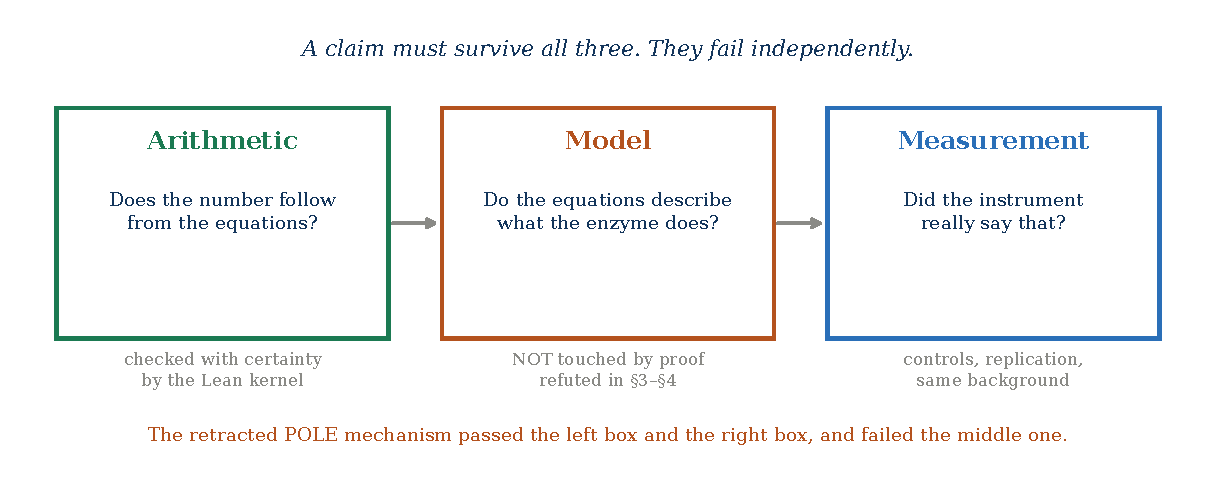
\includegraphics[width=\textwidth]{fig01_three_claims.pdf}
  \caption{The three independent ways a quantitative biological claim can fail.
  A proof assistant addresses the first box completely and the other two not at
  all. The organising case of this book passed the first and the third, and
  failed the second --- which is the only interesting way to be wrong.}
  \label{fig:threeclaims}
\end{figure}

\subsection{What the Lean kernel checks}

Throughout this book, theorems are checked by the Lean~4 proof assistant. It is
worth being exact about what that buys, because the rest of the book depends on
the distinction.

\begin{model}[The verification contract]\label{model:contract}
A Lean proof of a statement $H \Rightarrow C$ establishes: \emph{in every
situation where $H$ holds, $C$ holds}. It establishes nothing whatever about
whether $H$ holds in a cell.
\end{model}

Our gate is stricter than ``it compiled''. A file passes only if every declared
theorem carries a \lean{\#print axioms} line, no proof depends on \lean{sorryAx}
(Lean's marker for an admitted goal), and no proof invokes an axiom outside
$\{$\lean{propext}, \lean{Classical.choice}, \lean{Quot.sound}$\}$ --- the three
axioms of ordinary classical mathematics. A proof that quietly adds its own axiom
is rejected, because an axiom is just a way of assuming what you meant to prove.

\begin{remark}[Why bother, then?]
If proof cannot tell you about the cell, why formalise at all? Because of a
second-order effect that matters more than certainty: \emph{a hypothesis precise
enough to formalise is precise enough to refute}. Vague mechanisms are
unfalsifiable not because they are deep but because they are blurry. Section~3
proves a theorem whose entire value is that it has no free parameters --- and
Section~4 shows it failing against data. That failure is only possible because
the statement was sharp. This is the service formalisation renders in biology:
not certainty, but exposure.
\end{remark}

\subsection{A true theorem about a false model}

Here is the pattern that organises this book, in miniature. Consider the claim:

\begin{quote}
\emph{Variant $X$ removes two of the enzyme's three proofreading stages, so if
each stage discriminates by a factor $\gamma$, the error rate rises by $1/\gamma^2$.}
\end{quote}

The arithmetic is impeccable: if the error rate is $\gamma^m$ with $m$ stages,
then dropping from $m=3$ to $m=1$ multiplies it by $\gamma/\gamma^3 = \gamma^{-2}$.
At $\gamma = 1/100$ that is a factor of $10^4$. You can verify this in Lean, and
we do (Section~2, \lean{discrimination_gain}). The theorem is true.

The model is nevertheless false, and Section~3 proves that it must be --- not
mis-parameterised, but false for \emph{every} value of $\gamma$ and \emph{every}
number of stages. The arithmetic was never the weak point.

\begin{worked}[1.1: locating the error in a chain of reasoning]
A student presents the following argument and asks where, if anywhere, it fails.

\begin{enumerate}[label=(\roman*),leftmargin=*,itemsep=1pt]
  \item Error rate with $m$ stages is $\mathcal{E}_m = \gamma^m$, $\gamma \in (0,1)$.
  \item Variant $X$ has $m=1$; wild type has $m=3$.
  \item Therefore $\mathcal{E}_X/\mathcal{E}_{\mathrm{WT}} = \gamma^{-2}$.
  \item At $\gamma = 1/100$, variant $X$ is $10^4$ times more mutagenic.
  \item Tumours carrying $X$ should therefore show roughly $10^4$ times the mutation burden.
\end{enumerate}

\textbf{Analysis.} Steps (i), (iii) and (iv) are arithmetic and are correct. Step
(ii) is a modelling claim about what the variant does to the enzyme. Step (v) adds
a second modelling claim --- that mutation burden in a tumour is proportional to
the polymerase's intrinsic error rate, with nothing else intervening.

Both modelling steps turn out to be wrong, and they fail for \emph{different}
reasons. Step (ii) fails because of the no-go theorem of Section~3: an enzyme
that merely loses stages cannot be more mutagenic than one with no proofreading
at all, and $X$ is measured far above that bound. Step (v) fails because
mismatch repair sits between polymerase errors and fixed mutations, and
Section~5 shows that the measurements force that intervening step to be doing
something.

\textbf{Lesson.} ``Where is the error?'' is the wrong question when a chain mixes
arithmetic with modelling. The right question is: \emph{which steps could
conceivably have come out otherwise?} Only those steps carry evidence.
\end{worked}

\subsection{The epistemic ledger}

Every section of this book ends with a ledger in four columns.

\begin{itemize}[leftmargin=*,itemsep=1pt]
  \item \textbf{Measured} --- a number someone obtained from an instrument, with a citation.
  \item \textbf{Assumed} --- a modelling choice. It could have been made differently.
  \item \textbf{Proved} --- a consequence of the assumptions, checked by the kernel.
  \item \textbf{Open} --- what would settle the question and has not been done.
\end{itemize}

The discipline this enforces is simple: a claim may not migrate from
\emph{Assumed} to \emph{Proved} by being formalised. Formalising an assumption
proves its \emph{consequences}, never the assumption. Most of the overclaiming
in computational biology is exactly this migration, performed silently.

\begin{exercise}
For each statement, say whether it is arithmetic, modelling, or measurement, and
state what observation could falsify it.
\textbf{(a)} ``$\gamma^3 = 10^{-6}$ when $\gamma = 10^{-2}$.''
\textbf{(b)} ``Each proofreading stage acts independently.''
\textbf{(c)} ``The CAN1 forward-mutation rate of \texttt{pol2-4} is $44\times10^{-8}$.''
\textbf{(d)} ``Tumour mutational burden is proportional to polymerase error rate.''
\end{exercise}

\begin{exercise}
A colleague says: ``The result is machine-checked in Lean with zero \texttt{sorry}s,
so it cannot be wrong.'' Write a two-sentence reply that is accurate without being
dismissive of formalisation.
\end{exercise}

\begin{exercise}
Construct your own example of a true theorem about a false model, drawn from any
area of biology you know. State the theorem, state the modelling assumption that
fails, and state the measurement that would expose it.
\end{exercise}

\begin{ledger}
\textbf{Measured:} nothing in this section. \\
\textbf{Assumed:} that the three-way split --- arithmetic, model, measurement ---
is exhaustive for the claims this book considers. It is a didactic device, not a
theorem. \\
\textbf{Proved:} nothing in this section; the Lean content begins in Section~2. \\
\textbf{Open:} whether the discipline of the ledger generalises usefully beyond
the kind of mechanistic claim treated here.
\end{ledger}
